%!TEX program = xelatex
%# -*- coding: utf-8 -*-
%!TEX encoding = UTF-8 Unicode

\documentclass[12pt,oneside,a4paper]{article}\usepackage[]{graphicx}\usepackage[]{xcolor}
%% maxwidth is the original width if it is less than linewidth
%% otherwise use linewidth (to make sure the graphics do not exceed the margin)
\makeatletter
\def\maxwidth{ %
  \ifdim\Gin@nat@width>\linewidth
    \linewidth
  \else
    \Gin@nat@width
  \fi
}
\makeatother

\definecolor{fgcolor}{rgb}{0, 0, 0}
\newcommand{\hlnum}[1]{\textcolor[rgb]{0,0,0}{#1}}%
\newcommand{\hlstr}[1]{\textcolor[rgb]{0,0,1}{#1}}%
\newcommand{\hlcom}[1]{\textcolor[rgb]{0.443,0.478,0.702}{#1}}%
\newcommand{\hlopt}[1]{\textcolor[rgb]{0,0,0}{#1}}%
\newcommand{\hlstd}[1]{\textcolor[rgb]{0,0,0}{#1}}%
\newcommand{\hlkwa}[1]{\textcolor[rgb]{0.498,0,0.333}{\textbf{#1}}}%
\newcommand{\hlkwb}[1]{\textcolor[rgb]{0.498,0,0.333}{\textbf{#1}}}%
\newcommand{\hlkwc}[1]{\textcolor[rgb]{0.498,0,0.333}{\textbf{#1}}}%
\newcommand{\hlkwd}[1]{\textcolor[rgb]{0,0,0}{#1}}%

\usepackage{framed}
\makeatletter
\newenvironment{kframe}{%
 \def\at@end@of@kframe{}%
 \ifinner\ifhmode%
  \def\at@end@of@kframe{\end{minipage}}%
  \begin{minipage}{\columnwidth}%
 \fi\fi%
 \def\FrameCommand##1{\hskip\@totalleftmargin \hskip-\fboxsep
 \colorbox{shadecolor}{##1}\hskip-\fboxsep
     % There is no \\@totalrightmargin, so:
     \hskip-\linewidth \hskip-\@totalleftmargin \hskip\columnwidth}%
 \MakeFramed {\advance\hsize-\width
   \@totalleftmargin\z@ \linewidth\hsize
   \@setminipage}}%
 {\par\unskip\endMakeFramed%
 \at@end@of@kframe}
\makeatother

\definecolor{shadecolor}{rgb}{.97, .97, .97}
\definecolor{messagecolor}{rgb}{0, 0, 0}
\definecolor{warningcolor}{rgb}{1, 0, 1}
\definecolor{errorcolor}{rgb}{1, 0, 0}
\newenvironment{knitrout}{}{} % an empty environment to be redefined in TeX

\usepackage{alltt}
\usepackage{geometry}
\geometry{verbose,tmargin=2cm,bmargin=2cm,lmargin=2cm,rmargin=2cm}
\usepackage[pdfusetitle,
 bookmarks=true,bookmarksnumbered=true,bookmarksopen=true,bookmarksopenlevel=2,
 breaklinks=false,pdfborder={0 0 1},backref=false,colorlinks=false]
 {hyperref}
\hypersetup{pdfstartview={XYZ null null 1}}
\usepackage{url}
\setcounter{secnumdepth}{2}
\setcounter{tocdepth}{2}
\usepackage{microtype}

\usepackage{amsmath, amsthm, amssymb, amsfonts}
\usepackage[retainorgcmds]{IEEEtrantools}

\usepackage{algorithm}
\usepackage{algorithmic}
\renewcommand{\algorithmicrequire}{\textbf{Input:}} 
\renewcommand{\algorithmicensure}{\textbf{Output:}} 

\usepackage[sc]{mathpazo}
\linespread{1.1}
\usepackage[T1]{fontenc}


\usepackage{graphics}
\usepackage{graphicx}
\usepackage[figure]{hypcap}
\usepackage[hypcap]{caption}
\usepackage{tikz}
%\usepackage{grffile} 
%\usepackage{float} 
\usepackage{pdfpages}

\usepackage{multirow}
\usepackage{booktabs}
\usepackage{threeparttable}

%\usepackage[square,numbers,super,comma,sort]{natbib}
%\usepackage[backend=biber, style=nature, sorting=none, isbn=false, url=false, doi=false]{biblatex}
%\addbibresource{ref.bib}
%\usepackage[]{authblk}

\usepackage{verbatim}

\newcommand{\problem}[1]
{
    \clearpage
    \section*{Problem {#1}}
}

\newcommand{\subproblem}[1]
{
    \subsection*{Problem {#1}}
}


\newcommand{\solution}
{
    \vspace{15pt}
    \noindent\ignorespaces\textbf{\large Solution}\par
}

\usepackage{fancyhdr}
\usepackage{extramarks}
\lhead{\hmwkAuthorName}
\chead{\hmwkTitle}
\rhead{\firstxmark}
\cfoot{\thepage}

\newcommand{\hmwkTitle}{STAT 8051 HW 6}
\newcommand{\hmwkAuthorName}{Jingxiang Li}

\setlength\headheight{15pt}
\setlength\parindent{0pt}
\setlength{\parskip}{0.5em}

\newcommand{\m}[1]{\texttt{{#1}}}


\pagestyle{fancy}

\title{\hmwkTitle}
\author{\hmwkAuthorName}
\date{\today}
\IfFileExists{upquote.sty}{\usepackage{upquote}}{}
\begin{document}

\maketitle



\problem{12.5}
\emph{Donner party} (Data file: \m{Donner}) In the winter of 1846–1847, about 90 wagon train emigrants in the Donner party were unable to cross the Sierra Nevada Mountains of California before winter, and almost half of them starved to death. The data in file Donner from Johnson (1996) include some information about each of the members of the party. The variables include \m{age}, the age of the person; \m{sex}, whether male or female; \m{status}, whether the person was a member of a family group, a hired worker for one of the family groups, or a single individual who did not appear to be a hired worker or a member of any of the larger family groups; and \m{y}, a factor with levels died and survived.

\subproblem{12.5.1}
How many men and women were in the Donner Party? What was the survival rate for each sex? Obtain a test that the survival rates were the same against the alternative that they were different. What do you conclude?

\solution
\begin{knitrout}
\definecolor{shadecolor}{rgb}{1, 1, 1}\color{fgcolor}\begin{kframe}
\begin{alltt}
\hlkwd{require}\hlstd{(alr4)}
\hlstd{data} \hlkwb{<-} \hlkwd{na.omit}\hlstd{(Donner)}
\hlkwd{summary}\hlstd{(data}\hlopt{$}\hlstd{sex)}
\end{alltt}
\begin{verbatim}
## Female   Male 
##     35     53
\end{verbatim}
\end{kframe}
\end{knitrout}

As the result, there are 53 men and 35 women included in the Donner Party.

\begin{knitrout}
\definecolor{shadecolor}{rgb}{1, 1, 1}\color{fgcolor}\begin{kframe}
\begin{alltt}
\hlstd{tb_yVsSex} \hlkwb{<-} \hlkwd{table}\hlstd{(data}\hlopt{$}\hlstd{sex, data}\hlopt{$}\hlstd{y)}
\hlkwd{prop.table}\hlstd{(tb_yVsSex,} \hlnum{1}\hlstd{)}
\end{alltt}
\begin{verbatim}
##         
##               died  survived
##   Female 0.2857143 0.7142857
##   Male   0.5471698 0.4528302
\end{verbatim}
\end{kframe}
\end{knitrout}

As we can see, the survival rate is 71.4\% for female, and 45.3\% for male.

\begin{knitrout}
\definecolor{shadecolor}{rgb}{1, 1, 1}\color{fgcolor}\begin{kframe}
\begin{alltt}
\hlkwd{chisq.test}\hlstd{(tb_yVsSex,} \hlkwc{correct} \hlstd{=} \hlnum{FALSE}\hlstd{)}
\end{alltt}
\begin{verbatim}
## 
## 	Pearson's Chi-squared test
## 
## data:  tb_yVsSex
## X-squared = 5.8393, df = 1, p-value = 0.01567
\end{verbatim}
\end{kframe}
\end{knitrout}

Note that to test whether survival rates are the same for each sex is equivalent to test whether survival record and sex are independent, given the contingency table above. Hence we can apply $\chi^{2}$ test to the contingency table of \m{y} against \m{sex}. As the result, we have a p-value 0.01567, suggesting that we have enough evidence to reject the hypothesis that survival rates are the same for each sex, which means that survival rates are different for each sex.

\subproblem{12.5.2}
Fit the logistic regression model $\m{y} \sim \m{age}$, and provide an interpretation for the fitted coefficient for \m{age}.

\solution
\begin{knitrout}
\definecolor{shadecolor}{rgb}{1, 1, 1}\color{fgcolor}\begin{kframe}
\begin{alltt}
\hlstd{m1} \hlkwb{<-} \hlkwd{glm}\hlstd{(y} \hlopt{~} \hlstd{age,} \hlkwc{data} \hlstd{= data,} \hlkwc{family} \hlstd{=} \hlkwd{binomial}\hlstd{())}
\hlkwd{summary}\hlstd{(m1)}
\end{alltt}
\begin{verbatim}
## 
## Call:
## glm(formula = y ~ age, family = binomial(), data = data)
## 
## Deviance Residuals: 
##     Min       1Q   Median       3Q      Max  
## -1.5946  -1.2017   0.8436   0.9882   1.5765  
## 
## Coefficients:
##             Estimate Std. Error z value Pr(>|z|)   
## (Intercept)  0.97917    0.37460   2.614  0.00895 **
## age         -0.03689    0.01493  -2.471  0.01346 * 
## ---
## Signif. codes:  0 '***' 0.001 '**' 0.01 '*' 0.05 '.' 0.1 ' ' 1
## 
## (Dispersion parameter for binomial family taken to be 1)
## 
##     Null deviance: 120.86  on 87  degrees of freedom
## Residual deviance: 114.02  on 86  degrees of freedom
## AIC: 118.02
## 
## Number of Fisher Scoring iterations: 4
\end{verbatim}
\end{kframe}
\end{knitrout}

Note that \m{m1} is the logistic regression model $\m{y} \sim \m{age}$, and we see the estimated coefficient for \m{age} is $-0.03689$ with p-value 0.01346, suggesting that we have enough evidence to reject the hypothesis that it is zero. Since logit link function is used, we have 
$$\frac{p(x)}{1 - p(x)} = \mathrm{exp}(\beta^{'}x)$$
So that 1 unit increase in \m{age} will result in 0.03689 decrease in $log(\frac{p(x)}{1 - p(x)})$. In another word, if \m{age} increase by 1 unit, the odds of survival will decrease by about 1.3\%.

\subproblem{12.5.3}
Use your computer package to draw a scatterplot of the Pearson residuals from the model fit in Section 12.5 versus \m{age}. The residual plot will consist of two curves, with the curve of all positive values corresponding to survivors and the negative curve for deaths. As in Chapter 9, residual plots can be used to diagnose curvature, but this is quite hard without the aid of a smoother added to the plot.

\solution
\begin{knitrout}
\definecolor{shadecolor}{rgb}{1, 1, 1}\color{fgcolor}\begin{kframe}
\begin{alltt}
\hlkwd{require}\hlstd{(ggplot2)}
\hlstd{foo} \hlkwb{<-} \hlkwd{data.frame}\hlstd{(}\hlkwc{age} \hlstd{= data}\hlopt{$}\hlstd{age,} \hlkwc{residuals} \hlstd{= m1}\hlopt{$}\hlstd{residuals,} \hlkwc{survival} \hlstd{= data}\hlopt{$}\hlstd{y)}
\hlstd{p} \hlkwb{<-} \hlkwd{ggplot}\hlstd{(}\hlkwc{data} \hlstd{= foo)}
\hlstd{p} \hlkwb{<-} \hlstd{p} \hlopt{+} \hlkwd{geom_point}\hlstd{(}\hlkwd{aes}\hlstd{(}\hlkwc{x} \hlstd{= age,} \hlkwc{y} \hlstd{= residuals,} \hlkwc{shape} \hlstd{= survival),} \hlkwc{size} \hlstd{=} \hlnum{2}\hlstd{)}
\hlstd{p} \hlkwb{<-} \hlstd{p} \hlopt{+} \hlkwd{theme_bw}\hlstd{()} \hlopt{+} \hlkwd{theme}\hlstd{(}\hlkwc{text} \hlstd{=} \hlkwd{element_text}\hlstd{(}\hlkwc{size} \hlstd{=} \hlnum{14}\hlstd{))}
\hlstd{p} \hlkwb{<-} \hlstd{p} \hlopt{+} \hlkwd{ggtitle}\hlstd{(}\hlstr{"Residuals VS Age"}\hlstd{)}
\hlstd{p}
\end{alltt}
\end{kframe}

{\centering 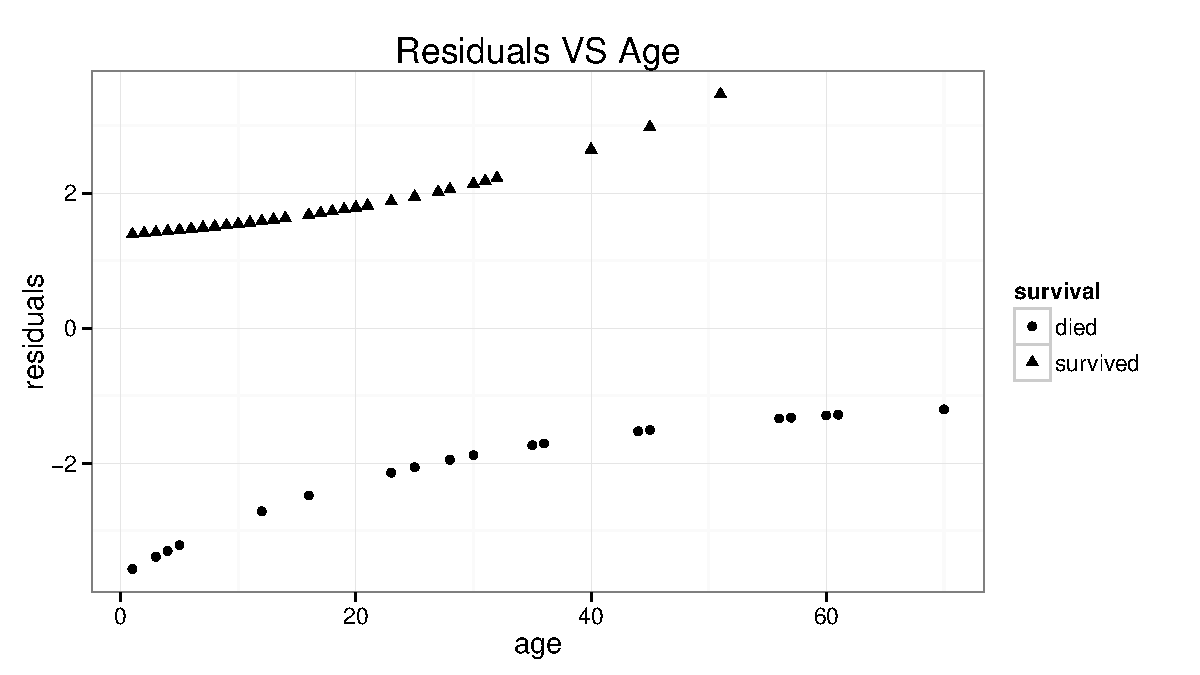
\includegraphics[width=.8\linewidth]{figure/p1253-1} 

}



\end{knitrout}

As we can see in the graph above, it's hard to say that the conditional variance of residuals given \m{age} is constant. In addition, the pattern of residuals against each \m{age} seems to suggest that there exists a nonlinear relationship between \m{y} and \m{age}, maybe we should include a polynomial term of \m{age} into the model.

\subproblem{12.5.4}
Fit the logistic regression model $\m{y} \sim \m{age} + \m{age} ^ 2 + \m{sex} + \m{status}$ and summarize results
\solution
\begin{knitrout}
\definecolor{shadecolor}{rgb}{1, 1, 1}\color{fgcolor}\begin{kframe}
\begin{alltt}
\hlstd{m2} \hlkwb{<-} \hlkwd{update}\hlstd{(m1,} \hlopt{~} \hlstd{age} \hlopt{+} \hlkwd{I}\hlstd{(age}\hlopt{^}\hlnum{2}\hlstd{)} \hlopt{+} \hlstd{sex} \hlopt{+} \hlstd{status)}
\hlkwd{summary}\hlstd{(m2)}
\end{alltt}
\begin{verbatim}
## 
## Call:
## glm(formula = y ~ age + I(age^2) + sex + status, family = binomial(), 
##     data = data)
## 
## Deviance Residuals: 
##     Min       1Q   Median       3Q      Max  
## -2.0431  -1.0391   0.5120   0.8664   2.0797  
## 
## Coefficients:
##                Estimate Std. Error z value Pr(>|z|)  
## (Intercept)   1.986e-01  6.172e-01   0.322   0.7476  
## age           1.675e-01  7.107e-02   2.357   0.0184 *
## I(age^2)     -3.889e-03  1.525e-03  -2.550   0.0108 *
## sexMale      -6.637e-01  5.588e-01  -1.188   0.2349  
## statusHired  -1.625e+00  7.481e-01  -2.173   0.0298 *
## statusSingle -1.852e+01  1.760e+03  -0.011   0.9916  
## ---
## Signif. codes:  0 '***' 0.001 '**' 0.01 '*' 0.05 '.' 0.1 ' ' 1
## 
## (Dispersion parameter for binomial family taken to be 1)
## 
##     Null deviance: 120.855  on 87  degrees of freedom
## Residual deviance:  92.363  on 82  degrees of freedom
## AIC: 104.36
## 
## Number of Fisher Scoring iterations: 16
\end{verbatim}
\end{kframe}
\end{knitrout}

Here we see the quadratic term of \m{age} is negative, suggesting that people with very small or very large age were more likely to die, and people about 22 years old had the maximized likelihood to survive. Then the coefficient for sex is negative, suggesting that women were more likely to survive than men. Lastly, the coefficients of \m{stautsHired} and \m{statusSingle} suggests that the person who was a member of a family group is more likely to survive, and the single individual who did not appear to be a hired worker or a member of any of the larger family groups is more likely to die.

\problem{12.6}
\emph{Challenger} (Data file: \m{Challeng}) These data from Dalal et al. (1989) records performance of O-rings for the 23 U.S. space shuttle missions prior to the Challenger disaster of January 20, 1986. For each of the previous missions, the temperature at takeoff and the pressure of a prelaunch test were recorded, along with the number of O-rings that failed out of 6.

Use these data to try to understand the probability of failure as a function of temperature, and of temperature and pressure. Use your fitted model to estimate the probability of failure of an O-ring when the temperature was $31^{\circ}F$, the launch temperature on January 20, 1986.

\solution
\begin{knitrout}
\definecolor{shadecolor}{rgb}{1, 1, 1}\color{fgcolor}\begin{kframe}
\begin{alltt}
\hlstd{data} \hlkwb{<-} \hlstd{Challeng}
\hlstd{m1} \hlkwb{<-} \hlkwd{glm}\hlstd{(}\hlkwd{cbind}\hlstd{(fail,} \hlnum{6} \hlopt{-} \hlstd{fail)} \hlopt{~} \hlstd{temp,} \hlkwc{family} \hlstd{= binomial,} \hlkwc{data} \hlstd{= data)}
\hlstd{m2} \hlkwb{<-} \hlkwd{update}\hlstd{(m1,} \hlopt{~} \hlstd{temp} \hlopt{+} \hlstd{pres)}
\hlkwd{anova}\hlstd{(m1, m2,} \hlkwc{test}\hlstd{=}\hlstr{"Chisq"}\hlstd{)}
\end{alltt}
\begin{verbatim}
## Analysis of Deviance Table
## 
## Model 1: cbind(fail, 6 - fail) ~ temp
## Model 2: cbind(fail, 6 - fail) ~ temp + pres
##   Resid. Df Resid. Dev Df Deviance Pr(>Chi)
## 1        21     18.086                     
## 2        20     16.565  1   1.5212   0.2174
\end{verbatim}
\begin{alltt}
\hlstd{foo} \hlkwb{<-} \hlkwd{data.frame}\hlstd{(}\hlkwc{temp} \hlstd{=} \hlnum{31}\hlstd{)}
\hlstd{tmp} \hlkwb{<-} \hlkwd{predict}\hlstd{(m1,} \hlkwc{newdata} \hlstd{= foo)}
\hlkwd{exp}\hlstd{(tmp)} \hlopt{/} \hlstd{(}\hlnum{1} \hlopt{+} \hlkwd{exp}\hlstd{(tmp))}
\end{alltt}
\begin{verbatim}
##         1 
## 0.8177744
\end{verbatim}
\end{kframe}
\end{knitrout}

Here we establish two logistic regression models \m{m1} and \m{m2}, where \m{m1} has temperature as the only regressor, \m{m2} has temperature and pressure as regressors. Then we compare these two models by $\chi^{2}$ test. The resulting p-value derived from $\chi^{2}$ test suggests that there is no significant difference between these two models, hence we choose the smaller one \m{m1}. 

Then we make prediction about failure probability by \m{m1}, given temperature as $31^{\circ}F$, the resulting predicted probability is 81.7\%.

\problem{12.7}
\emph{Titanic} (Data file: \m{Whitestar}) The Titanic was a British luxury passenger liner that sank when it struck an iceberg about 640 km south of Newfoundland on April 14–15, 1912, on its maiden voyage to New York City from Southampton, England. Of 2201 known passengers and crew, only 711 are reported to have survived. These data from Dawson (1995) classify the people on board the ship according to their \m{sex} as male or female; \m{age}, either child or adult; and \m{class}, either first, second, third, or crew. Not all combinations of the three-factors occur in the data, since no children were members of the crew. For each age/sex/class combination, the number of people \m{m} and the number surviving \m{Surv} are also reported. The data are shown in Table 12.8.

\subproblem{12.7.1}
Fit a logistic regression model with terms for factors \m{sex}, \m{age}, and \m{class}. On the basis of examination of the data in Table 12.8, explain why you expect that this mean function will be inadequate to explain these data.

\solution
\begin{knitrout}
\definecolor{shadecolor}{rgb}{1, 1, 1}\color{fgcolor}\begin{kframe}
\begin{alltt}
\hlstd{data} \hlkwb{<-} \hlstd{Whitestar}
\hlstd{m1} \hlkwb{<-} \hlkwd{glm}\hlstd{(}\hlkwd{cbind}\hlstd{(surv, m} \hlopt{-} \hlstd{surv)} \hlopt{~} \hlstd{class} \hlopt{+} \hlstd{age} \hlopt{+} \hlstd{sex,}
          \hlkwc{data} \hlstd{= data,} \hlkwc{family} \hlstd{= binomial)}
\hlkwd{summary}\hlstd{(m1)}
\end{alltt}
\begin{verbatim}
## 
## Call:
## glm(formula = cbind(surv, m - surv) ~ class + age + sex, family = binomial, 
##     data = data)
## 
## Deviance Residuals: 
##     Min       1Q   Median       3Q      Max  
## -4.1356  -1.7126   0.7812   2.6800   4.3833  
## 
## Coefficients:
##             Estimate Std. Error z value Pr(>|z|)    
## (Intercept)   1.1862     0.1586   7.480 7.40e-14 ***
## classfirst    0.8577     0.1573   5.451 5.00e-08 ***
## classsecond  -0.1604     0.1738  -0.923    0.356    
## classthird   -0.9201     0.1486  -6.192 5.93e-10 ***
## agechild      1.0615     0.2440   4.350 1.36e-05 ***
## sexmale      -2.4201     0.1404 -17.236  < 2e-16 ***
## ---
## Signif. codes:  0 '***' 0.001 '**' 0.01 '*' 0.05 '.' 0.1 ' ' 1
## 
## (Dispersion parameter for binomial family taken to be 1)
## 
##     Null deviance: 671.96  on 13  degrees of freedom
## Residual deviance: 112.57  on  8  degrees of freedom
## AIC: 171.19
## 
## Number of Fisher Scoring iterations: 5
\end{verbatim}
\end{kframe}
\end{knitrout}

From Table 12.8 we can see that almost all females survived, except for those in the third class, where over half of the women died. This suggests that at least there should be an interaction between \m{sex} and \m{class}.

\subproblem{12.7.2}
Fit a logistic regression model that includes all the terms of the last part, plus all the two-factor interactions. Use appropriate testing procedures to decide if any of the two-factor interactions can be eliminated. Assuming that the mean function you have obtained matches the data well, summarize the results you have obtained by interpreting the parameters to describe different survival rates for various factor combinations. (Hint: How does the survival of the crew differ from the passengers? First class from third class? Males from females? Children versus adults? Did children in first class survive more often than children in third class?)

\solution
\begin{knitrout}
\definecolor{shadecolor}{rgb}{1, 1, 1}\color{fgcolor}\begin{kframe}
\begin{alltt}
\hlstd{m2} \hlkwb{<-} \hlkwd{update}\hlstd{(m1,} \hlopt{~} \hlstd{(class} \hlopt{+} \hlstd{age} \hlopt{+} \hlstd{sex)} \hlopt{^} \hlnum{2}\hlstd{)}
\hlkwd{Anova}\hlstd{(m2)}
\end{alltt}
\begin{verbatim}
## Analysis of Deviance Table (Type II tests)
## 
## Response: cbind(surv, m - surv)
##           LR Chisq Df Pr(>Chisq)    
## class       120.73  3  < 2.2e-16 ***
## age          20.34  1  6.486e-06 ***
## sex         359.37  1  < 2.2e-16 ***
## class:age    37.26  2  8.101e-09 ***
## class:sex    65.01  3  4.984e-14 ***
## age:sex       1.69  1     0.1942    
## ---
## Signif. codes:  0 '***' 0.001 '**' 0.01 '*' 0.05 '.' 0.1 ' ' 1
\end{verbatim}
\end{kframe}
\end{knitrout}

First we use Anova to see the significance of each main effects and interactions. As the result, it seems that the interaction between \m{age} and \m{sex} is not significant, suggesting that there might be no interaction between these two predictors. Then let's see the coefficients for this model.

\begin{knitrout}
\definecolor{shadecolor}{rgb}{1, 1, 1}\color{fgcolor}\begin{kframe}
\begin{alltt}
\hlkwd{summary}\hlstd{(m2)}
\end{alltt}
\begin{verbatim}
## 
## Call:
## glm(formula = cbind(surv, m - surv) ~ class + age + sex + class:age + 
##     class:sex + age:sex, family = binomial, data = data)
## 
## Deviance Residuals: 
##         1          2          3          4          5          6          7          8  
## 0.000e+00  0.000e+00  7.563e-07  1.021e-05  0.000e+00  0.000e+00  2.216e-06  1.190e-05  
##         9         10         11         12         13         14  
## 1.238e-07  0.000e+00  0.000e+00  1.075e-07  0.000e+00  0.000e+00  
## 
## Coefficients: (1 not defined because of singularities)
##                        Estimate Std. Error z value Pr(>|z|)    
## (Intercept)           1.897e+00  6.191e-01   3.064  0.00218 ** 
## classfirst            1.658e+00  8.003e-01   2.072  0.03826 *  
## classsecond          -8.004e-02  6.876e-01  -0.116  0.90732    
## classthird           -2.055e+00  6.385e-01  -3.218  0.00129 ** 
## agechild             -3.625e-02  3.932e-01  -0.092  0.92655    
## sexmale              -3.147e+00  6.245e-01  -5.039 4.68e-07 ***
## classfirst:agechild   2.536e+01  8.377e+04   0.000  0.99976    
## classsecond:agechild  2.752e+01  7.087e+04   0.000  0.99969    
## classthird:agechild          NA         NA      NA       NA    
## classfirst:sexmale   -1.136e+00  8.205e-01  -1.385  0.16616    
## classsecond:sexmale  -1.068e+00  7.466e-01  -1.431  0.15254    
## classthird:sexmale    1.664e+00  6.560e-01   2.536  0.01120 *  
## agechild:sexmale      6.868e-01  5.254e-01   1.307  0.19116    
## ---
## Signif. codes:  0 '***' 0.001 '**' 0.01 '*' 0.05 '.' 0.1 ' ' 1
## 
## (Dispersion parameter for binomial family taken to be 1)
## 
##     Null deviance: 6.7196e+02  on 13  degrees of freedom
## Residual deviance: 2.5128e-10  on  2  degrees of freedom
## AIC: 70.621
## 
## Number of Fisher Scoring iterations: 24
\end{verbatim}
\end{kframe}
\end{knitrout}

As the result, we can see that people in the first class are more likely to survive than crews, and the crews' likelihood of surviving are almost the same as second class people's likelihood, people in the third class are the most poor ones with the lowest likelihood of surviving. Females are more likely to survive than males in general, but in the third class males' likelihood of surviving is more than females'. There is no evidence showing that children are more likely to survive than adults. Then Children in the first class survive more often than children in the third class. 
\end{document}
